\section{Fast Fourier Transform\label{sec:fft}}
The DFT is not a hard sum to calculate,
but naively computing it for $k \in [0;N)$ will take $O(N^2)$ time.
By exploiting certain redundancies,
we can recursively factorize the sum in such a way that it can be computed in $O(N \log N)$ time.
An algorithm that takes advantage of such factorizations is called a Fast Fourier Transform (FFT).

A comprehensive explanation of FT, DFT, and FFT can be found in \cite{fft}.
This book uses the Cooley-Tukey algorithm,
but we will use a different factorization for simplicity and brevity.

\subsection{Twiddle factor}
Before we get into the factorization, let us abstract away some complexity.
To simplify the representation and computation of the DFT,
we define what is often referred to as the \textit{twiddle factor}:
\begin{equation}
    W_N = e^{-i 2 \pi / N}
\end{equation}
Using this, we can then rephrase the DFT as:
\begin{equation}
    X(k) = \sum_{n = 0}^{N - 1} W_N^{nk} x(n)
\end{equation}
\begin{figure}
    \centering
    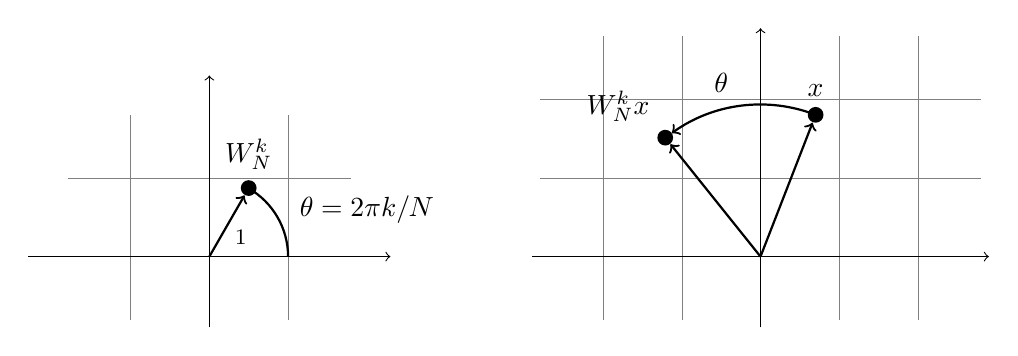
\begin{tikzpicture}
        \draw[step=1, gray, very thin] (-1.8, -0.8) grid (1.8, 1.8);
        \draw[->] (-2.3,0) -- (2.3,0) coordinate (x axis);
        \draw[->] (0,-0.9) -- (0,2.3) coordinate (y axis);
        \node (unit) at (0.4, 0.25){\footnotesize 1};
        \node (w) at (0.5, 0.87)[circle, fill=black, minimum size=2mm, inner sep=0mm, label=above:$W_N^k$]{};
        \node (theta) at (2,0.6){$\theta = 2 \pi k/N$};
        \path[thick, ->, draw] (0,0) -- (w);
        \draw[thick] (1,0) arc[radius = 1, start angle=0, end angle=60];

        \draw[step=1, gray, very thin] (4.2, -0.8) grid (9.8, 2.8);
        \draw[->] (4.1,0) -- (9.9,0) coordinate (x axis);
        \draw[->] (7,-0.9) -- (7,2.9) coordinate (y axis);
        \node (x) at (7.7, 1.8) [circle, fill=black, minimum size=2mm, inner sep=0mm, label=above:$x$]{};
        \node (wx) at (5.79,1.51)[circle, fill=black, minimum size=2mm, inner sep=0mm, label=above left:$W_N^k x$]{};
        \draw[thick, ->] (7,0) -- (x);
        \draw[thick, ->] (7,0) -- (wx);
        \draw[thick, ->] (7.7, 1.8) arc[radius = 1.93, start angle=68.75, end angle=125.75];
        \node (theta2) at (6.5, 2.2){$\theta$};
    \end{tikzpicture}
    \caption{Representing the twiddle factor in the complex plane.
    The factor itself is a unit vector with angle $\theta$.
    Multiplying some $x$ by this number is equivalent to rotating $x$ by $\theta$.\label{fig:twid}}
\end{figure}
The twiddle factor can viewed as a rotation of the complex number $1 + 0i$
around $0 + 0i$ in the complex plane, scaled by $1/N$.
Multiplying some complex number $x$ by $W_N^k$
will thus rotate $x$ by an angle of $\theta = 2 \pi \cdot k/N$ (see figure \ref{fig:twid}).
As such, we can compute twiddle factors by
\begin{equation}
    W_N^k = \cos \theta + i \sin \theta,~~\theta = 2\pi k/N
\end{equation}

As a result of being a rotated unit vector,
the twiddle factor has certain properties that we can exploit.
Namely, it wraps around after a full rotation,
taking its negative is equivalent to making a half rotation,
and upscaling $k$ by some constant $c$ is the same as downscaling $N$ by $1/c$.
These properties can be formally expressed as follows:
\begin{align}
    \textbf{Periodicity:} &~~W^k_N = W^{k + N}_N\\
    \textbf{Symmetry:}    &~~W^{k + N/2}_N = -W^k_N\\
    \textbf{Scaling:}     &~~W_N^{ck} = W_{N/c}^{k}
\end{align}
Having observed these, we can now move on to the factorization.

\subsection{Factorization}
There are numerous different ways in which the DFT sum can be factorized.
They all have the same $O(N \log N)$ time complexity,
but differ in the concrete amount of operations that they require.
In the interest of simplicity,
we adapt a factorization presented in \cite{brunton}.
FFT factorizations are traditionally expressed in matrix form,
but this factorization is simple enough that we can skip that step.
Note that the factorization as presented only works for inputs of length $N = 2^\gamma$.

The first step of the factorization
is to split the input list $x$ into even- and odd-indexed elements:
\begin{align}
    &x_\textit{even} = \langle x_{2n} ~|~ n \in [0; N/2) \rangle\\
    &x_\textit{odd}  = \langle x_{2n + 1} ~|~ n \in [0; N/2) \rangle
\end{align}
%
Next, we define the DFTs of these new lists.
Using the scaling property of the twiddle factor,
we can express these DFTs using $W_N^{2nk}$ rather than $W_{N/2}^{nk}$:
\begin{align}
    X_\textit{even}(k) &= \sum_{n = 0}^{N/2 - 1} W_{N/2}^{nk} x_\textit{even}(n) = \sum_{n = 0}^{N/2 - 1} W_{N}^{2nk} x(2n) \\
    X_\textit{odd}(k) &= \sum_{n = 0}^{N/2 - 1} W_{N/2}^{nk} x_\textit{odd}(n) = \sum_{n = 0}^{N/2 - 1} W_{N}^{2nk} x(2n + 1)
\end{align}

Now we can reformulate $X(k)$ using $X_\textit{even}$ and $X_\textit{odd}$.
We split the sum into sums of even- and odd-indexed elements,
factor out a coefficient of the odd sum,
and then substitute:
\begin{align}
    X(k) &= \sum_{n = 0}^{N - 1} W_N^{nk} x(n) \\
    &= \sum_{n = 0}^{N/2 - 1} W_N^{2nk} x(2n) + \sum_{n = 0}^{N/2 - 1} W_N^{(2n + 1)k} x(2n + 1) \\
    &= \sum_{n = 0}^{N/2 - 1} W_N^{2nk} x(2n) + W_N^k \sum_{n = 0}^{N/2 - 1} W_N^{2nk} x(2n + 1) \\
    &= X_\textit{even}(k) + W_N^k X_\textit{odd}(k)
\end{align}
%
In order to achieve our $O(N \log N)$ goal,
we only wish to compute $X_\textit{even}(k)$ and $X_\textit{odd}(k)$ for $k \in [0;N/2)$.
To still compute $X(k)$ for $k \in [N/2;N)$, we exploit the periodicity of the twiddle factor.
Since $W_{N/2}^{k + N/2} = W_{N/2}^k$, we also have $X_\textit{even}(k + N/2) = X_\textit{even}(k)$.
Thus we can ``wrap around'' for the upper half of $X$:
\begin{equation}
    X(k) =
    \begin{cases}
        X_\textit{even}(k) + W_N^k X_\textit{odd}(k) &\text{if}~k \in [0;N/2) \\
        X_\textit{even}(k') + W_N^{k} X_\textit{odd}(k') &\text{if}~k \in [N/2;N) ~\text{where}~k' = k - N/2
    \end{cases}
\end{equation}
%
The last step
\begin{itemize}
    \item halves the number of multiplications,
    \item allows us to trivially compute the FFT in-place,
    \item and defines the FFT in such a way that it can be directly inverted.
\end{itemize}

From the symmetry property of the twiddle factor, we get $W_N^k = -W_N^{k - N/2} = -W_N^{k'}$.
Because of this,
we can multiply the odd DFT by the same coefficient when computing the lower and upper DFT of $X$.
This gives us the final factorization:
\begin{equation}
    X(k) =
    \begin{cases}
        X_\textit{even}(k) + W_N^k X_\textit{odd}(k) &\text{if}~k \in [0;N/2) \\
        X_\textit{even}(k') - W_N^{k'} X_\textit{odd}(k') &\text{if}~k \in [N/2;N) ~\text{where}~k' = k - N/2
    \end{cases}
\end{equation}
This factorization can be recursively applied
until we have divided our input into pieces of size 1.
Conveniently, the DFT of $\langle v \rangle$ is simply $\langle v \rangle$,
so this makes for a simple base case.

\subsection{Algorithm}
With the factorization in place,
we can construct an algorithm to compute the FFT:

\begin{algorithm}[H]
    \setstretch{1.2}
    \DontPrintSemicolon
    \caption{$\textsc{FFT}(x, N)$}
    \KwIn{Discrete uniformly spaced signal $x$ with size $N = 2^\gamma$.}
    \KwOut{Discrete Fourier Transform of $x$.}
    Let $x_\textit{even} = \langle x(2n) ~|~ n \in [0;N/2) \rangle$\;
    Let $x_\textit{odd} = \langle x(2n + 1) ~|~ n \in [0;N/2) \rangle$\;
    Let $X_\textit{even} = \textsc{FFT}(x_\textit{even}, ~N/2)$\;
    Let $X_\textit{odd} = \textsc{FFT}(x_\textit{odd}, ~N/2)$\;
    \For{$k\gets0$ \KwTo $N/2 - 1$}{
        Let $o = W_N^k X_\textit{odd}(k)$\;
        $X_\textit{even}(k) \leftarrow X_\textit{even}(k) + o$\;
        $X_\textit{odd}(k) \leftarrow X_\textit{even}(k) - o$\;
    }
    \KwRet{$\langle X_\textit{even}, X_\textit{odd}\rangle$}
\end{algorithm}

The algorithm performs two recursive calls with sizes $N/2$.
Then it performs $O(N)$ work to combine the results.
We can thus prove the time bound with a recursive formula:
\begin{equation}
    T(N) = O(N) + 2T(N/2) = O(N \log N)
\end{equation}
Now that we have a general overview of the algorithm,
we can move on to the subject of reversibility.
